\documentclass{RPI-SIW}

% Load any necessary packages here
\usepackage[OT1]{fontenc}
\usepackage{graphicx,xcolor}
\usepackage{lipsum}
\usepackage{amsmath}
\usepackage{amsfonts}
\usepackage{amssymb}

% Author and affiliation declaration
\author{
	% Author 1
	Jane J. Doe\textsuperscript{1}\textsuperscript{*}
	and 
	% Author 2
	John L. Doe\textsuperscript{2};
	% First affiliation
	\textsuperscript{1}First affiliation (organization name \& address),
	% Second affiliation
	\textsuperscript{2}Second affiliation (organization name \& address).
	% Email for POC (currently the first author)
	\textsuperscript{*}[email address for corresponding author if desired]
}

% Title (it will be forced to all caps)
\title{Extended Abstract Title}

% Event title for the bottom left footer
\event{2\textsuperscript{nd} RPI Space Imaging Workshop. Saratoga Springs, NY. \\ 28-30 October 2019}


\begin{document}

% Build the custom title from the class file
\maketitle

% Custom abstract environment
\MakeAbstract{
	A brief narrative abstract describing the topic, its importance, its relationship to the field of space imaging, and key results/findings. This summary should allow a reader to determine if the rest of the extended abstract is of interest. This brief abstract must not exceed 100 words.
}

\section*{Introduction}
Every extended abstract must begin with an introduction section. This section should explain the problem being solved and provide the background/context to fully frame the problem.

\section*{Formatting Guidelines}
The entire extended abstract is expected to be around 750--1,500 words.  The body of the extended abstract is 9.5pt \LaTeX\ Computer Modern font, approximately equivalent in size to 10pt Times New Roman. Text appears in a two-column format and paragraphs are justified. Each page is standard US Letter (8.5''x11'') with 1'' margins on all sides.

The extended abstract, including references, may be no more than two pages. As this is an imaging workshop, an additional third page with supplemental images may be provided at the author’s discretion \cite{christian2012}.

\section*{Heading Styles}
Top-level heading styles are bolded and end with a period. Each word in the heading is capitalized. Headings should be descriptive phrases and not complete sentences. The format for second-level headings follows immediately:

\subsection*{Styling of a Second-Level Heading}
Second-level headers are italic. The formatting is essentially the same as the top-level heading, except it is italicized instead of bolded \cite{owen2008}.

\section*{Figures and Tables}
Include figures and tables as necessary.  Captions go below figures and above tables.  Captions should be bold italic. An example is in Fig.~\ref{figs::dione}.

\section*{Submission Format}
All extended abstracts should be submitted online through the webform on the workshop website. Uploads must be submitted as PDF files.

\section*{Lorem Ipsum}
\lipsum[1-2]

\begin{figure}[h]
	\centering
	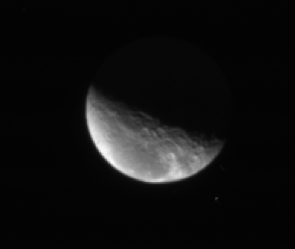
\includegraphics[width=0.29\textwidth]{figs/Dione.png}
	\caption{Image of Dione from Cassini \cite{porco2005}.}
	\label{figs::dione}
\end{figure}

\lipsum[3-3]

\section*{References}
References should be listed in the order in which they appear. List the DOI for each reference where it is available. We suggest the following format (you may use common journal abbreviations in cases where a DOI is provided): 

\bibliographystyle{ieeetr}
\renewcommand{\refname}{}
\vspace*{-5pt}\hspace*{-10pt}
\parbox{\linewidth}{\footnotesize \bibliography{bib}}

\end{document}